\documentclass[12pt]{article}
\usepackage{geometry}
\geometry{left=1in,right=0.75in,top=1in,bottom=1in}
\newcommand{\Problem}{A}
\newcommand{\Team}{2307532}
\usepackage{newtxtext}
\usepackage{booktabs}
\usepackage{indentfirst}
\usepackage{amsmath,amssymb,amsthm}
\usepackage{newtxmath} % must come after amsXXX
\usepackage{siunitx}
\usepackage[pdftex]{graphicx}
\usepackage{xcolor}
\usepackage{fancyhdr}
\usepackage{appendix}
\lhead{Team \Team}
\rhead{}
\cfoot{}

\newtheorem{theorem}{Theorem}
\newtheorem{corollary}[theorem]{Corollary}
\newtheorem{lemma}[theorem]{Lemma}
\newtheorem{definition}{Definition}
\setlength{\headheight}{14.49998pt}

\begin{document}
\graphicspath{{.}}  % Place your graphic files in the same directory as your main document
\DeclareGraphicsExtensions{.pdf, .jpg, .tif, .png}
\thispagestyle{empty}
\vspace*{-16ex}
\centerline{\begin{tabular}{*3{c}}
	\parbox[t]{0.3\linewidth}{\begin{center}\textbf{Problem Chosen}\\ \Large \textcolor{red}{\Problem}\end{center}}
	& \parbox[t]{0.3\linewidth}{\begin{center}\textbf{2023\\ MCM/ICM\\ Summary Sheet}\end{center}}
	& \parbox[t]{0.3\linewidth}{\begin{center}\textbf{Team Control Number}\\ \Large \textcolor{red}{\Team}\end{center}}	\\
	\hline
\end{tabular}}

\begin{center}

%标题
\section*{
    The Fungi: The Expert of Carbon Cycle Balance
}

%summary
\subsection*{summary}
\end{center}
%摘要开始
%代码两个换行代表PDF一个换行
%quotation环境换行自动缩进两格
%使用\\换行不会产生缩进
%\textbf{}加粗
\begin{quotation}
    %摘要正文
    Decomposition of organic matters by \textbf{fungi}, an indispensable part of carbon cycle, can
    make carbon reused in the environment. A recent article explores the impact of different
    traits on its decomposition effeciency. In this paper, we focus on two main traits, hyphal
    extension rate and moisture tolerance, together with \textbf{interactions} among fungi and various
    environmental conditions, to simulate the breakdown of woody fibers and comprehend the
    importance of \textbf{biodiversity}.


    Our \textbf{GAME} model is made up of the initials of four task names. 
    Before we start our ex- periments, we build up a prediction 
    model to simulate the cross action among different fungi and 
    their effect on the decomposition process of woody ibers. 
    We adopt Gause’s Competitive Model to uncover the interactions 
    among species and derive a differential system by considering 
    the change of woody ibers amount. The model describes growth, 
    hyphal extension, competition, and decomposition of fungi.

    Firstly, in order to simplify the model, we ix temperature $T=\qty{22}{\degreeCelsius}$, 
    and set the trait parameters of three different fungi artiicially. 
    Experiment results shown that our model is of high reasonability since 
    the predicted decomposition rate is nearly 30\%, 
    which approximately equals to veriied research results.
{\tiny }
   %关键字
    \textbf{keywoed}:Decomposition Rate, Multi-environment, Gause’s Model
    \end{quotation}
%摘要结束    


    


% to here
\clearpage
\pagestyle{fancy}
\tableofcontents 
\contentsname
\newpage
\setcounter{page}{1}
\rhead{Page \thepage\ }
\section{Introduction}
\subsection{Background}
Example: The main task of the repeater is to amplify the received signal and transmit it further forward \cite{Gyaourova2002,MaLZhangY2021}. As repeaters can be added to the radio network to improve the overall coverage and capacity of the system\cite{PRASAD2014}, they have played a significant role in high frequency radio spectrum propagation\cite{Gyaourova2002}. However, repeater location has less flexibility due to infrastructural, environmental, and governmental issues and rules.
\begin{enumerate}
    \item Applying CTCSS technology, the interferences are canceled
    \item Deploying the minimum number of repeaters
    \item Accommodating enough simultaneous users
\end{enumerate}

\subsection{Our work}
kdfsdhfoidshfdsfffffffffsaddddddddddfs
dfghdfsgdfgdfgdhasukfh
sahdfkhsdkjfhkhdsf
rgregstretwertsdfjagdktretgeraerfds
\paragraph{Task1}
ryryryfgdg

sgdsg%空行 换行

\paragraph{Task2}
ryryry

sgrdrgsd
\paragraph{Task3}
ryryry

fdfgasdfasdffaewfeasf

\subsection{Data Pre-processiong}
erewafsdfeadf fwefdds fsfs dase ds aef efsd e fads feaf sadf e
df sdf efasd gae asdga sefd sdgea fd gs gs
rg rg rd rgds frs dfg rsdf  \ref{T1}.


%三线表的画法
\begin{table}[!htbp] 
		\centering%居中环境
	\caption{111}\label{T1}%标题

\begin{tabular}{llll}
	\toprule %添加表格头部粗线
	fasf & dsfae & efea  & efaf \\
	\hline %绘制一条水平横线
	212  & fsdf1 & efsfd & dfd  \\
	32   & 2434  & efs   & fsf  \\
	\bottomrule %添加表格底部粗线
\end{tabular}
\end{table}

\section{Assumptions}
We make the following assumptions to complete our model through this paper. Furthermore, improvements of these simplified assumptions will be achieved later.
\begin{itemize}
    \item First item
    \item Second item
    \item Third item
\end{itemize}


\section{Notations}

Add your text here. We use the … in Table \ref{T2}. 

\begin{table}[!htbp] 
\centering

\caption{Three Line Table}\label{T2}
\begin{tabular}{lll} %需要10列

\toprule %添加表格头部粗线
A  &  B  &  C\\
\hline %绘制一条水平横线
AAAAAAAAAA  &  B  &  C\\

A  &  B  &  C\\
\bottomrule %添加表格底部粗线
\end{tabular}
\end{table}

\section{Data Processing}
In statistics, the lack of data is very common in the dataset and may cause certain bias in the conclusion. Therefore, data imputation is necessary to eliminate such bias and obtain more concrete results. Through preliminary observation on the dataset, we find that some are missing and garbled data, which has an important impact on the analysis of the problem. Therefore, we first distinguish the anomalous information from the database and then process the missing data. We use the method of deleting by list to do data interpolation.
\begin{equation}
    a^2 + b^2 = c^2
    \end{equation}
    \begin{equation}
        r=density*\pi*g^2
        \end{equation}

\section{Model I: XXXXX}
\subsection{Description of XXXX}
The interaction between influencers and followers is like the relationship between individuals in social networks, so we build a network of musicians' mutual influence based on existing social network analysis. Before constructing the model, let us introduce some definitions and concepts that will be used in this paper. 

\begin{figure}[h]
\centering
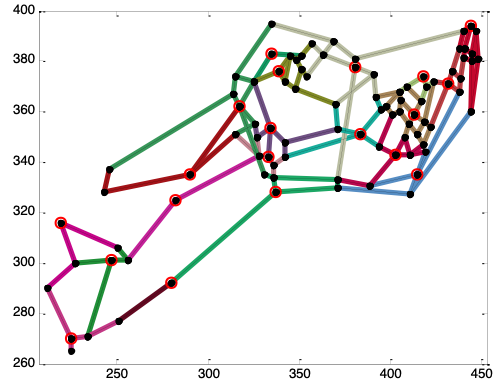
\includegraphics{fig1.png}
\caption{Title of picture}
\end{figure}


A network or graph is a set of nodes (also called vertices) connected via links (also called edges). Networks connected by directed links are called directed networks while networks connected by undirected edges are called undirected networks[1]. In order to take a decision about the network structure we have measured the following graph parameters.

Degree: The degree $k$ of a vertex $i$  is the number of connections of that vertex and   is the average of   over all the vertices of the network.
Average shortest path: Two vertices   and   are connected if one can go from  to following the edges in the graph. The path from   to   may not be unique. The minimum path distance or geodesic path   is the shortest path distance from   to  . The average shortest path over every pair of vertices is
\begin{equation}
    f(x)=\dfrac{\sin x}{1+\cos x},
\end{equation}
where $x$ is number. For an  equation without reference, no tag is needed, as 
$$F(X)=\int_a^b g(x) dx.$$

\subsection{	XXX model }

e.g. Genre influence model based on cosine similarity Add your text here.

\subsection{XXX Results} 
Add your text here.
\section{Model II: XXXXX}

Add your text here.

\section{Model Analysis}
\subsection{Sensitivity Analysis}
\subsubsection{XXXX}

Add your text here.

\subsubsection{XXXX}
Add your text here.

\subsection{Strengths and Weaknesses}
Add your text here.

\section{	Conclusions}
Add your text here. 


\bibliographystyle{plain}
\bibliography{mcmbib}

\newpage
\addcontentsline{toc}{section}{APPENDIX}
\section*{APPENDIX} 

\appendix

We put what here.

\section{Source code}

Put source code here.
\section{Source code for Model X}

Put source code here.

%%%%%%%%%%%%%%%%%%%%%%%%%%%%%%
\end{document}
\end